\documentclass[a4paper,10pt]{report}
\usepackage[utf8]{inputenc}
\usepackage{algorithm}
\usepackage{algorithmic}
\usepackage{graphicx}

\begin{document}

\section*{\textit{Layered Label Propagation}}

  A principal ideia dos algoritmos de \textit{Label Propagation} seguem um padrão comum. Estes algoritmos consistem num conjunto de iterações e no início é atribuído a cada vértice uma \textit{label} que representa o \textit{cluster} a que pertence. No início do algoritmo, cada vértice tem uma \textit{label} diferente. O critério de atribuição da \textit{label},a cada vértice, é o que diferencia os vários algoritmos de \textit{Label Propagation}. Um dos algoritmos mais conhecidos é o \textit{Standard Label Propagation}, em que a regra de atribuição da \textit{label} a um vértice é a \textit{label} que ocorrer mais frequentemente na sua vizinhança. 
  
  Uma outra variante, denominada \textit{Absolute Pott Model}, indica que a \textit{label} que é atribuída ao vértice é a que maximiza a seguinte equação: 
 
  \begin{center}
    \begin{equation}
      \label{apmeq}
      ki-\gamma(vi-ki)
    \end{equation}
  \end{center}    
  
  Sendo, $ki$ os vértices na vizinhança que têm a $label_i$ e $v_i$ todos os vértices que têm a $label_i$.
  Este algoritmo pode ser descrito da seguinte forma:
  
  \begin{algorithm}
    \caption{\textit{Absolute Pott Model}}\label{apmalg}
    \begin{enumerate}
    \item Obter uma permutação do grafo.
    \item Iniciar todos os vértices atribuindo uma \textit{label} única e por $v_i=1$ para cada $label_i$ .
    \item Iterar sobre a permutação obtida e para todas as \textit{labels} na vizinhança de cada vértice ver qual é maximizada pela equação \ref{apmeq} e atribuir ao vértice essa \textit{label}. Decrementar $v_i$ para a \textit{label} antiga e incrementar o $v_i$ correspondente à nova \textit{label}.
    \end{enumerate}
  \end{algorithm}

  Ambos os algoritmos apresentados anteriormente têm alguns problemas. O \textit{Standard Label Propagation} tende a produzir um \textit{clusters} de grandes dimensões(contendo a maior parte dos vértices) e o \textit{Absolute Pott Model} tem o problema de não se saber à partida o valor ideal para $\gamma$.
  
  Baseado no algoritmo \textit{Standard Label Propagation} surgiu o \textit{Layered Label Propagation}. Este algoritmo consiste no seguinte:
  
  \begin{algorithm}
    \caption{\textit{Layered Label Propagation}}\label{llpalg}
    \begin{enumerate}
    \item Para cada iterações chamar o Algoritmo \ref{apmalg} tendo $gama$ valores compreendidos dentro do seguinte conjunto: $\{0\}\cup\{2^{{-}i},i=0,...,K\} $.
    \item Com o \textit{output} resultante da chamada ao Algoritmo \ref{apmalg}, ordenar os vértices de modo a que os que tenham a mesma \textit{label} fiquem próximos. Para vértices que estejam na mesma comunidade (têm a mesma \textit{label}) é mantida a sua ordem.
    \end{enumerate} 
  \end{algorithm}
      
  \begin{figure}
    \center
    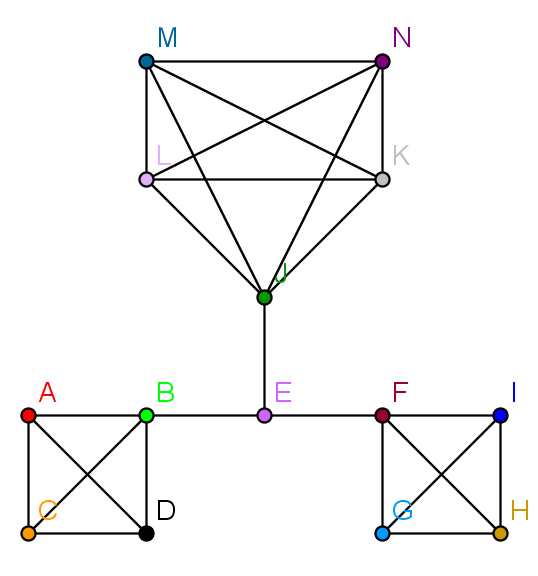
\includegraphics{graph_step0.png}
    \caption{Grafo de exemplo em que cada vértice foi-lhe atribuída uma \textit{label}(cor) inicial que é única.}
    \label{graph0llp}
  \end{figure}
  
  \paragraph{Exemplo} Para o grafo(Figura \ref{graph0llp}) pode-se calcular de forma sequencial o Layered Label Propagation, para cada iteração $i$, começando por se fazer uma permutação($\pi_i$) dos vértices do grafo e itera-los por essa ordem. 
  
  Neste exemplo quando haver mais do que uma \textit{label} com resultados iguais resultantes da equação \ref{apmeq} e que a maximizem então é escolhida aquela a que pertence ao menor vértice. Neste contexto as labels estão a ser representadas por cores será daí ser dada uma maior importância à comunidade que tem o vértice com menor ordem lexicográfica.

  Para $i=1$ admite-se que $\pi_1=$[M,E,L,G,F,H,D,C,K,N,J,B,A,I], $\gamma=1$(para facilitar) e que $v_i$=1 para todas as \textit{label}. Segundo o algoritmo \ref{apmalg} segue-se a iteração sobre $\pi_1$ e para cada vértice vê-se qual a \textit{label} que maximiza a equação \ref{apmeq}. 
  Nesta primeira iteração para qualquer vértice o resultado da equação \ref{apmeq} referente à sua \textit{label} não é o valor que maximiza porque $k_i=0$ e o mesmo acontece para as \textit{labels} que não se encontram na vizinhança, daí a omissão destes elementos. 
  \\[0.25cm]
  Para M:\\
  \begin{itemize}
   \item $label_l = k_l - \gamma ( v_l - k_l ) = 1 - 1 ( 1 - 1) = 1$
   \item $label_n = k_n - \gamma ( v_n - k_n ) = 1 - 1 ( 1 - 1) = 1$
   \item $label_k = k_k - \gamma ( v_k - k_k ) = 1 - 1 ( 1 - 1) = 1$
   \item $label_j = k_j - \gamma ( v_j - k_j ) = 1 - 1 ( 1 - 1) = 1$
  \end{itemize}
  M junta-se a J.
  
  
  
  
\section*{\textit{Layered Label Propagation} Distribuído}
  
  
\end{document}
